\documentclass[a4paper]{article}

\usepackage{amsfonts}
\usepackage{amsmath}
\usepackage[affil-it]{authblk}
\usepackage[margin=1in]{geometry}
\usepackage{graphicx}
\usepackage{hyperref}
\usepackage{mathrsfs}
\usepackage{tikz}

\usepackage{clrscode}

\usetikzlibrary{shapes}

\setlength{\parskip}{3pt}

\DeclareGraphicsExtensions{.pdf}

\begin{document}
    \title{One-Way Quantum Communication Complexity}
    \author{Dominic Moylett\thanks{\texttt{\href{dominic.moylett@bristol.ac.uk}{dominic.moylett@bristol.ac.uk}}}}
    \affil{Quantum Engineering Centre for Doctoral Training,\\University of Bristol}
    \date{\today}
    \maketitle

    \begin{abstract}
        Communication complexity is the study of how much information two or more parties need to share with each other in order to perform joint computation of a problem. There are many benefits to this model of computation, from many lower bound proofs to applications in cryptography and data streaming. In this report, we will summarise the most exciting recent trends in the one-way form of quantum communication complexity, look at what quantum advantages already exist and what problems are still open.
    \end{abstract}

    \section{Introduction}

    \section{Communication Complexity}

        Communication complexity was developed by Yao in 1979 as an analysis of distributed computing \cite{Yao:1979:CQR:800135.804414}. Under this model of computation, our computation is done between two parties, commonly referred to as Alice and Bob, with inputs $x, y \in \{0, 1\}^n$, respectively. The two parties do not know each other's inputs; Alice does not know $y$ and Bob does not know $x$. Alice and Bob then exchange a series of messages between each other through a protocol established before computation, with their aim being to jointly compute $f(x, y)$. The question communication complexity asks is how many bits of information do Alice and Bob need to communicate in order for the two of them to compute a solution. We offer a sketch of a typical communication complexity problem in Figure~\ref{fig:cc}.

        A na\"{i}ve solution to any communication complexity problem can be completed using $n$ bits of communication: Alice sends $x$ to Bob and Bob then does all of the computation for $f(x, y)$. So the question then becomes if it is possible to compute $f(x, y)$ with $o(n)$ bits of communication.

        \begin{figure}
            \centering
            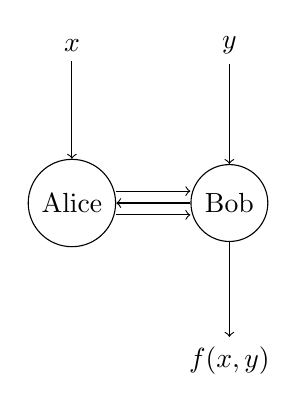
\begin{tikzpicture}[->, draw, node distance=2cm]
                \node[circle, draw] (Alice) at (0,0) {Alice};
                \node[circle, draw] (Bob) [right of=Alice] {Bob};
                \node (x) [above of=Alice] {$x$};
                \node (y) [above of=Bob] {$y$};
                \node (bout) [below of=Bob] {$f(x, y)$};
                \path
                    (x) edge (Alice)
                    (y) edge (Bob)
                    (Bob) edge (bout);
                \path ([yshift=1ex]Alice.east) edge ([yshift=1ex]Bob.west);
                \path (Bob.west) edge (Alice.east);
                \path ([yshift=-1ex]Alice.east) edge ([yshift=-1ex]Bob.west);
            \end{tikzpicture}
            \caption{An example of communication complexity. Alice and Bob begin computation with bit strings $x$ and $y$. They then exchange a series of messages based on a pre-determined protocol. Computation completes when Bob outputs $f(x, y)$.}
            \label{fig:cc}
        \end{figure}

        In quantum communication complexity, first proposed in 1993 by Yao \cite{366852}, we also have parties Alice and Bob given inputs $x$ and $y$, respectively, and have to produce $f(x, y)$ for some function $f$. But now our two parties can send quantum messages between each other, and the complexity is measured in the number of qubits that are communicated.

        Another model by Burhman and Cleve \cite{quant-ph/9704026} does not use the physical sending of data between the parties, but instead uses the measurement of entangled particles for remote computation. Our focus for this report however will be on the former. Note that it is possible to simulate this model by the ability to communicate quantum states: Alice generates entangled pairs of qubits and sends one of the pair to Bob. Likewise, it is possible to simulate communicating $l$ qubits by use of $l$ entangled pairs and $2l$ classical bits of communication, via quantum teleportation \cite{PhysRevLett.70.1895}.

        \subsection{One-Way Communication Complexity}

        A specific subset of communication complexity, which we will focus on throughout this report, is one-way communication complexity. In this model of computation, Alice and Bob again receive respective inputs $x, y \in \{0, 1\}^n$ with the aim of Bob being able to output $f(x, y)$ for some function $f$. The difference now is that only one message is allowed to be sent, from Alice to Bob. This is illustrated in \ref{fig:ow-cc}.

        Like general communication complexity, one-way communication complexity can also be solved na\"{i}vely in $n$ bits of communication by Alice sending $x$ to Bob. So once again, our question is if we can do better with less communication.

        \begin{figure}
            \centering
            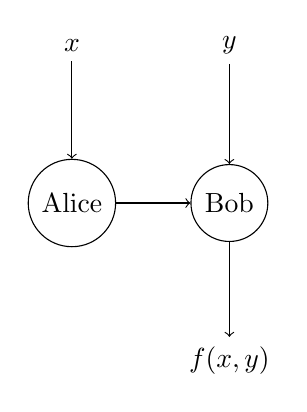
\begin{tikzpicture}[->, draw, node distance=2cm]
                \node[circle, draw] (Alice) at (0,0) {Alice};
                \node[circle, draw] (Bob) [right of=Alice] {Bob};
                \node (x) [above of=Alice] {$x$};
                \node (y) [above of=Bob] {$y$};
                \node (bout) [below of=Bob] {$f(x, y)$};
                \path
                    (x) edge (Alice)
                    (y) edge (Bob)
                    (Bob) edge (bout);
                \path (Alice.east) edge (Bob.west);
            \end{tikzpicture}
            \caption{An example of one-way communication complexity. Alice receives input $x$ and Bob receives input $y$. Alice then sends a single message to Bob. Using this additional information from Alice, Bob performs and outputs the computation $f(x, y)$.}
            \label{fig:ow-cc}
        \end{figure}

        \subsection{Holevo's Theorem}

        Even before Yao's work on the formalisation of Communication Complexity, it was clear that quantum communication would not be able to speed up some problems. In particular, a consequence of Holevo's theorem \cite{Hol73}, meant that while a message of $n$ bits could be compressed into a message of at most $n-1$ qubits, the same message could not be retrieved from said qubits. We phrase this as a one-way communication complexity problem below.

        \begin{codebox}
            \Procname{Problem $\proc{COMMUNICATION}$}
            \zi \const{Alice's input:} $x \in \{0, 1\}^n$.
            \zi \const{Bob's input:} none.
            \zi \const{Bob's output:} $x$.
        \end{codebox}

        By Holevo's theorem, we know that the above problem requires Alice to send $\Omega(n)$ qubits to Bob. A later proof by Nayak \cite{814608} shows that if we compress a message of $n$ bits into a message of $m < n$ qubits, the probability that we can successfully retrieve all $n$ bits again is at most $2^{m-n}$. This can be seen if we create an encoding $x \mapsto \{q_{x,i}|\phi_{x_i}\rangle\}$ such that $x$ is an $n$-bit string and $\{q_{x,i}|\phi_{x_i}\rangle\}$ is a mixed state over $m$ qubits. We decode this message by measuring over projection operators $\{P_x\}$. The mean probability of Bob successfully decoding an $x$ that has been selected uniformly at random is $2^{-n}\sum_{x, i}q_{x, i}\|P_x|\phi_{x,i}\rangle\|^2$. This can be bounded by making our states pure and setting $|\phi_x\rangle = \max_{|\psi_{x, i}\rangle}\|P_x|\phi_{x, i}\rangle\|^2$:

        $$\frac{1}{2^n}\sum_{x, i}q_{x, i}\|P_x|\phi_{x,i}\rangle\|_2^2 \leq \frac{1}{2^n}\sum_{x}\|P_x|\phi_{x}\rangle\|_2^2$$

        Next, we decompose $P_x$ into an orthonormal basis $\{|\hat{e}_{x, j}\rangle\}$ and create a subspace $E$ that spans the code words $\{|\phi_x\rangle\}$ with projection $Q$:

        $$\frac{1}{2^n}\sum_{x}\|P_x|\phi_{x}\rangle\|_2^2 = \frac{1}{2^n}\sum_{x, j}\langle\phi_x|\hat{e}_{x, j}\rangle\langle\hat{e}_{x, j}|\phi_x\rangle \leq \frac{1}{2^n}\sum_{x}\|Q|\hat{e}_{x, j}\rangle\|_2^2$$

        Finally, we decompose $Q = \sum_i|e_i\rangle\langle e_i|$ where $\{|e_i\rangle\}$ is an orthonormal basis spanning $E$. Note that since $|phi_x\rangle$ is conveyed in at most $m$ qubits, $|\{|e_i\rangle\}| \leq 2^m$. Hence we conclude that

        $$\frac{1}{2^n}\sum_{x}\|Q|\hat{e}_{x, j}\rangle\|_2^2 \leq \frac{1}{2^n}\sum_{x, j, i}|\langle e_i|e_{x, i}\rangle \leq \frac{1}{2^n}\sum_{i}\|e_i\|_2^2 \leq 2^{m - n}.$$

        As a result, if Alice sends fewer qubits to Bob, the probability of them successfully communicating a classical message decreases exponentially, and the only case where they succeed all of the time is when $m = n$. The only exception to this is when Alice and Bob have shared entangled qubits between each other prior to computation, in which case superdense coding can be used to send two bits by sending one qubit \cite{PhysRevLett.69.2881}. Brassard \cite{quant-ph/0101005} explains that if we have unlimited entanglement between Alice and Bob then we can only at most reduce the amount of communication by a factor of $1/2$, as quantum teleportation can be used to send qubits from one party to the other using entangled pairs and communicating with classical bits \cite{PhysRevLett.70.1895}.

        Holevo's Theorem has in turn led to communication complexity problems which cannot be solved more efficiently with quantum communication. One example of this is the Inner Product problem, studied in \cite{Cleve201311}:

        \begin{codebox}
            \Procname{Problem $\proc{INNER-PRODUCT}$}
            \zi \const{Alice's input:} $x \in \{0, 1\}^n$.
            \zi \const{Bob's input:} $y \in \{0, 1\}^n$.
            \zi \const{Bob's output:} $\sum_{i = 0}^{n - 1}x_i.y_i (\textrm{mod} 2)$.
        \end{codebox}

        Cleve et al.~showed that if we were able to solve this problem in less than $O(n)$ qubits of communication, then it would be possible for Alice to communicate $x$ to Bob in $o(n)$ qubits, thus violating Holevo's theorem. A summary of this proof is given in \cite{RevModPhys.82.665}.

        While it is clear that we cannot solve all problems in fewer qubits than we can in classical bits, we will in the next two sections look at more specific problems which we can solve by communication of fewer qubits.

    \section{Functions}

        \subsection{Distributed Deutsch-Jozsa}

        The Distributed Deutsch-Jozsa problem, first introduced by Buhrman, Cleve and Wigderson \cite{Buhrman:1998:QVC:276698.276713}, was the first example of an exponential separation between quantum and classical computation complexity. The problem, and its quantum protocol as described in Buhrman et al.~\cite{RevModPhys.82.665}, are stated as follows, where $\mathcal{D}(x, y)$ is the Hamming distance between $x$ and $y$ and $U_x = \sum_{i=0}^{n-1}(-1)^{x_i}|i\rangle\langle i|$ for $x \in {0, 1}^n$:

        \begin{codebox}
            \Procname{Protocol $\proc{DISTRIBUTED DEUTSCH-JOZSA}$}
            \zi \const{Alice's input:} $x \in \{0, 1\}^n$.
            \zi \const{Bob's input:} $y \in \{0, 1\}^n$.
            \zi \const{Promise:} $x = y$ or $\mathcal{D}(x, y) = n/2$.
            \zi \const{Bob's output:} $0$ iff $x = y$, $1$ otherwise.
            \li Alice starts computation in the $|0\rangle^{\otimes \log n}$ state and applies $U_xH^{\otimes \log n}$ to get the state $|\psi\rangle$.
            \li Alice sends $|\psi\rangle$ to Bob.
            \li Bob applies $H^{\otimes \log n}U_y$ and measures in the computational basis.
            \li Bob outputs $0$ if they measure $|0\rangle^{\otimes \log n}$ and 1 otherwise.
            \End
        \end{codebox}

        The state Alice sends to Bob is $|\psi\rangle = \frac{1}{\sqrt{n}}\sum_{i=0}^{n-1} (-1)^{x_i}|i\rangle$. When Bob applies $U_y$ to this state, they end up with the state $\frac{1}{\sqrt{n}}\sum_{i=0}^{n-1}(-1)^{x_i}(-1)^{y_i}|i\rangle$. We'll now consider this state for two situations: one where $x = y$ and one where they differ in $n/2$ places, denoted $|\psi_0\rangle$ and $|\psi_1\rangle$, respectively.

        Note that if $x = y$ then $(-1)^{x_i}(-1)^{y_i} = 1$, so $|\psi_0\rangle = \frac{1}{\sqrt{n}}\sum_{i = 0}^{n-1}|i\rangle$. $|\psi_1\rangle$ on the other hand will have exactly $n/2$ amplitudes which are positive, and $n/2$ amplitudes which are negative. From this we can see that $\langle\psi_0|\psi_1\rangle = \frac{n/2 - n/2}{n} = 0$, so the states can be distinguished from one another upon measurement. Finally, Bob's application of $H^{\otimes \log n}$ converts their state to the computational basis. Note that $H|\psi_o\rangle = |0\rangle^{\otimes\log n}$, so measuring this state will indicate that $x = y$ and any other state will indicate that $\mathcal{D}(x, y) = n/2$.

        So we have been able to deterministically solve this problem with $O(\log n)$ qubits of communication between Alice and Bob. How much classical communication is required to solve it? One common way of lower bounding deterministic communication protocols for a function $f$ is to partition the problem space up into rectangles $(a, b, c, d)$ such that $f(x_i, y_i) = f(x_i', y_i')$ for any pair of inputs $(x_i, y_i), (x_i', y_i') \in \{x_a,x_{a + 1},...,x_{b}\} \times \{y_c, y_{c+1},...,y_d\}$. We can lower bound the number of messages to $c$ bits if we need $2^c$ rectangles to cover the entire problem space.

        For this problem, we will focus on the inputs $(x, x)$, where $x$ is an $n$-bit string with hamming weight $n/2$. There are $\binom{n}{n/2} \approx 2^n/\sqrt{n}$ such inputs, which means that at least one rectangle $R$ must contain $2^{n-c}/\sqrt{n}$ of these inputs. Because $DDJ(x, x) = 0 ~\forall~x\in \{0, 1\}^n$, all $(x, y)$-pairs in $R$ must satisfy either $x = y$ to output $0$ or $\mathcal{D}(x, y) \neq n/2$ to break the promise. Characteristic analysis detailed in \cite{RevModPhys.82.665} show that the maximum number of $(x, x)$ inputs in $R$ is $1.99^n$ \cite{frankl1987forbidden}. Hence we have the inequality

        $$\frac{2^{n-c}}{\sqrt{n}} \leq 1.99^n$$

        Solving for $c$ shows that $c \geq \log_2(2^n/1.99^n\sqrt{n}) = \Omega(0.007n)$. Note that Buhrman et al.~\cite{RevModPhys.82.665} provide this as a lower bound instead of an asymptotic lower bound, but this is only correct if $n \geq 728$. A plot of $\log_2(2^n/1.99^n\sqrt{n})/n$ for even values of $n$ ranging from $2$ to $998$ is given in Appendix \ref{sec:ddj-lower-bound}.

        Thus we have an exponential gap between deterministic classical communication and quantum communication for the Distributed Deutsch-Jozsa problem. However, this quantum advantage is lost when compared to randomised classical computation for some positive integer $c$:

        \begin{codebox}
            \Procname{Protocol $\proc{DISTRIBUTED DEUTSCH-JOZSA}$}
            \li Alice picks $c$ unique items $a \in \{0, 1\}^n$ uniformly at random.
            \li Alice sends $(a_i, x_{a_i})~ \forall i \in \{0,...,c-1\}$.
            \li Bob returns $0$ if $x_{a_i} = y_{a_i}~ \forall i \in \{0,...,c-1\}$, and $1$ otherwise.
            \End
        \end{codebox}

        Bob always returns $0$ if $x = y$, so our protocol has no true negative results. If $\mathcal{D}(x, y) = n/2$, then the protocol fails if $x_{a_i} = y_{a_i} \forall i \in \{0,...,c-1\}$, which happens with probability $1/2^c$. Finally, note that each $a_i$ can be communicated in $\log n$ bits, so the overall communication required is $c(\log n + 1)$ bits.

        \subsection{Subgroup Membership}
        \label{sec:subgroup-membership}

        One disadvantage of the Distributed Deutsch-Jozsa problem that we saw above is that a quantum protocol has no advantage over a randomised classical protocol. Another disadvantage is that the problem is a {\em partial function}, in that it requires a {\em promise} on the input: that either the two bit strings are identical or they differ in exactly $n/2$ places. This promise results in a very contrived problem with little practical application. This begs the question: Are there any functions which do not rely on promises that yield a quantum advantage under the communication complexity model -- better known as {\em total functions}?

        Sadly, no significant gap has been shown for total functions in the one-way model, even though two-way communication has shown polynomial gaps \cite{Buhrman:1998:QVC:276698.276713}, and other models such as Simultaneous Message Passing have shown exponential gaps \cite{PhysRevLett.87.167902}. But there are some problems which have shown potential. Aaronson et al.~\cite{0902.3175} were the first to explore the problem of subgroup membership as potentially yielding a quantum advantage in the one-way comunication complexity setting. Their protocol for solving subgroup membership, based on an earlier quantum algorithm by Watrous \cite{Watrous:2000:SQP:795666.796590}, is described below, where $G$ is a group, $\mathscr{H}_G$ is the set of all subgroups of $G$, $|+\rangle = \frac{1}{\sqrt{2}}(|0\rangle + |1\rangle)$ and $U_{G, y} = \sum_{g \in G}|yg\rangle\langle g|$ for some $y \in G$:

        \begin{codebox}
            \Procname{Protocol $\proc{SUBGROUP-MEMBERSHIP}$}
            \zi \const{Alice's input}: $H \in \mathscr{H}_G$.
            \zi \const{Bob's input}: $y \in G$.
            \zi \const{Bob's output}: $1$ if $y \in H$, $0$ otherwise.
            \li Alice prepares the state $|H\rangle = \frac{1}{\sqrt{|H|}}\sum_{h \in H}|h\rangle$, which is then sent to Bob.
            \li Bob prepends an ancilla qubit to get $|H\rangle|+\rangle$ and applies $U_{G, y}$ controlled on the final qubit.
            \li Bob applies a Hadamard to the second qubit and measures in the computational basis.
        \end{codebox}

        Any element $h \in H$ can be described in $\lceil\log |G|\rceil$ bits, so Alice needs to send $O(\log |G|)$ qubits to Bob in order to perform this protocol.

        After line 2, Bob has the state $\frac{1}{\sqrt{2}}(|H\rangle|0\rangle + |yH\rangle|1\rangle)$, where $|yH\rangle = \frac{1}{\sqrt{|H|}}\sum_{yh \in H}|h\rangle$. If $y \in H$ then $yh \in H~ \forall h \in H$, so $|yH\rangle = |H\rangle$. Therefore, if $y \in H$ then $U_{G, y}|H\rangle|+\rangle = |H\rangle|+\rangle$, so applying a Hadamard to the final qubit makes the final qubit $|0\rangle$. A measurement in the computational basis will thus always yield $0$.

        On the other hand, if $y \notin H$ then $\langle yH|H\rangle = 0$, so applying the Hadamard produces

        $$\frac{1}{2}(|H\rangle|0\rangle + |H\rangle|1\rangle + |yH\rangle|0\rangle - |yH\rangle|1\rangle).$$

        Measuring the final qubit will result in $|0\rangle$ -- and thus a false positive -- with probability $1/2$. We can repeat this protocol a constant number of times to get a negligible error probability.

        Classically, it has been shown by Miltersen et al.~\cite{Miltersen199837} that any one-way randomised protocol with completeness probability of $1/2$ and perfect soundness must use $\Omega(\log|G|)$ bits of communication. Aaronson et al.~\cite{0902.3175} have conjectured that this bound still holds even if we relax soundness to $1/3$ and tighten completeness to $2/3$.

        So, if we can find a total subgroup membership function that cannot classically be solved using $O(\log |G|)$ bits of communication, then we will have a polynomial gap between classical and quantum communication for a total function. The problem is that there are many subgroup membership problems which {\em can} be solved classically within these constraints. One example is that of normal subgroups. Aaronson et al.~\cite{0902.3175} showed that this problem can be solved with error probability of $1/2$ using only $O(\log |G|)$ bits of communication.

        To explain this classical protocol, we first need to describe complex characters. For any complex field representation $\rho$ of $G$, the complex character $\chi$ is the function $\chi(g) = \textrm{tr}(\rho(g))~\forall~g\in G$. For any two elements $g, g' \in G$, we have the relation that $\chi(gg'g^{-1}) = \chi(g)$. $\chi(1)$ is the dimension of $\rho$, and the kernel of $\chi$, denoted $\textrm{ker}(\chi) = \{g \in G|\chi(g) = chi(1)\}$. If $\rho$ is irreducible then $\chi$ is an irreducible character, and the set of irreducible complex characters of $G$ is denoted $\textrm{Char}(g)$. Finally, if $H$ is a normal subgroup of $G$, then let

        $$\Lambda_H = \{\chi \in \textrm{G}|H\subseteq \textrm{ker}(\chi)\}.$$

        Finally, given this definition we note that

        $$\sum_{\chi \in \Lambda_H}[\chi(1)]^2 = \frac{|G|}{|H|}.$$

        We now describe the protocol from Aaronson et al.~\cite{0902.3175}:

        \begin{codebox}
            \Procname{Protocol $\proc{NORMAL-SUBGROUP-MEMBERSHIP}$}
            \zi \const{Alice's input}: $H \in \mathscr{H}_G$ such that $H$ is normal.
            \zi \const{Bob's input}: $y \in G$.
            \zi \const{Bob's output}: $1$ if $y \in H$, $0$ otherwise.
            \li Alice chooses a random complex character $\mu$ such that $H \subseteq \textrm{ker}(\mu)$ with probability $\frac{|H|}{|G|}[\mu(1)]^2$.
            \li Alice sends $\mu$ to Bob.
            \li Bob outputs $1$ if $y \in \textrm{ker}(\mu)$ and $0$ otherwise.
        \end{codebox}

        If $y \in H$ then $y \in \textrm{ker}(\mu)$, so $\mu(y) = \mu(1)$ and thus the protocol will always correctly report a member of $H$. So now we only need to consider the case where the $y \notin H$ yet the protocol accepts. This will occur if Alice picks a character $\mu$ such that $y \in \textrm{ker}(\mu)$. We shall call the set of all characters that would cause an error $B$. Based on Alice's selection criteria, the probability of an error is thus

        $$\frac{|H|}{|G|}\sum_{\chi \in B}[\chi(1)]^2.$$

        To analyse this further, we will look at the smallest normal subgroup of $G$ which contains both $H$ and $y$. We will call this subgroup $K$, which can be stated formally as $K = \{gkg^{-1}|g \in G, k \in H \cup \{y\}\}$. Note that $|K| \geq 2|H|$, as $\forall~h\in H, h \in K$ and $hyh^{-1} \in K$, but $hyh^{-1} \notin H$.

        The final point we will need is that $B \subseteq \Lambda_K$. Consider a character $\chi \in B$. Because $\chi$ could be selected by Alice, we know that $H \subseteq \textrm{ker}(\chi)$, and also that $y \in \textrm{ker}(\chi)$ because $\chi \in B$. We can conclude from this that any other element in $K$ must also be in $\textrm{ker}(\chi)$, as $\chi(gkg^{-1}) = \chi(k)~\forall~g\in G, k\in H \cup \{y\}$. Thus $K \subseteq \textrm{ker}(\chi)$ and we can conclude that $\chi \in \Lambda_K$.

        Using the above points, we can show that

        $$\frac{|H|}{|G|}\sum_{\chi \in B}[\chi(1)]^2 \leq \frac{|H|}{|G|}\sum_{\chi \in \Lambda_K}[\chi(1)]^2 = \frac{|H|}{|G|}\frac{|G|}{|K|} \leq \frac{|H|}{|G|}\frac{|G|}{2|K|} = \frac{1}{2}.$$

        Thus this protocol fails with probability at most $1/2$. Finally, we note that is is possible to describe a character $\mu$ sent from Alice to Bob in $\lceil\log|G|\rceil$ bits, as $\mu \in \Lambda_H$ and $|\lambda_H| \leq |Char(G)| \leq |G|$, so this protocol only needs $O(\log |G|)$ classical bits of communication. So in order to find a subgroup membership problem which provides an exponential gap between random and quantum computation, we need to consider non-normal subgroups.

        \subsection{Hidden Matching}
        \label{sec:hidden-matching}

        A matching $M$ is a sequence of pairs $(i_1, j_1), (i_2, j_2),...,(i_k, j_k) \in [n]^2$. If no integer appears in any pair more than once, then the pairs are {\em disjoint}. A matching is said to be {\em partial} the pairs are disjoint but some indexes do not appear in any pair, and {\em perfect} if each integer appears in exactly one pair. A matching $M$ together with an $n$-bit string $x$ define a $k$-bit string as follows:

        $$Mx = (x_{i_1} \oplus x_{j_1}), (x_{i_2} \oplus x_{j_2}), ... (x_{i_k} \oplus x_{j_k})$$

        The Hidden Matching problem was first investigated in terms of one-way communication complexity in \cite{doi:10.1137/060651835}. The problem and its quantum protocol are defined below, where $\mathcal{M}_n$ is the set of perfect matchings on $n$-node graphs:

        \begin{codebox}
            \Procname{Protocol $\proc{HIDDEN-MATCHING}$}
            \zi \const{Alice's input}: $x \in \{0,1\}^n$.
            \zi \const{Bob's input}: $M \in \mathcal{M}_n$.
            \zi \const{Bob's output}: $(i, j, x_i\oplus x_j)$ for some $(i, j) \in M$.
            \li Alice prepares the state $|x\rangle = \frac{1}{\sqrt{n}}\sum_{i = 0}^{n - 1}(-1)^{x_i}|i\rangle$, which is then sent to Bob.
            \li Bob measures $|x\rangle$ in the $\{\frac{1}{\sqrt{2}}(|i\rangle\pm|j\rangle)|(i, j) \in M\}$ basis and gets the state $|\psi_{i\pm j}\rangle$.
            \li Bob returns $(i, j, b)$, where $b = 0$ if $|\psi_{i\pm j}\rangle = \frac{\pm 1}{\sqrt{2}}(|i\rangle+|j\rangle)$ and $b = 1$ if $|\psi_{i\pm j}\rangle = \frac{\pm 1}{\sqrt{2}}(|i\rangle-|j\rangle)$.
        \end{codebox}

        First, note that since $M$ is a perfect matching, each index $i \in \{0,...,n-1\}$ occurs in exactly one $(i, j)$-pair in $M$. Thus the inner product of any two different states in the basis in step 2 of the above protocol is

        $$\langle\psi_{i\pm j}|\psi_{i'\pm j'}\rangle = \frac{\langle i|i'\rangle \pm \langle i|j'\rangle \pm \langle j|i'\rangle \pm \langle j|j'\rangle}{2} = 0$$

        The only exception is comparing the states $|\psi_{i + j}\rangle$ and $|\psi_{i - j}\rangle$, where:

        $$\langle\psi_{i + j}|\psi_{i - j}\rangle = \frac{\langle i|i\rangle - \langle j|j\rangle}{2} = 0$$

        Hence this basis is orthogonal and can be measured. The probability of measuring $|\psi_{i \pm j}\rangle$ is

        $$P(i\pm j) = \left|\frac{1}{\sqrt{n}}\sum_{k=0}^{n-1}(-1)^{x_k}\frac{1}{\sqrt{2}}(|i\rangle \pm |j\rangle)\right|^2 = \frac{|(-1)^{x_i} \pm (-1)^{x_j}|^2}{2n}$$.

        Note that if $x_i \oplus x_j = 0$ then $x_i = x_j$, so $P(i-j) = \frac{1}{2n}(1-1) = 0$ and thus Bob will only measure the state $|\psi_{i+j}\rangle$. Likewise, if $x_i \oplus x_j = 1$ then $P(i+j) = \frac{1}{2n}(1-1) = 0$, so Bob will only measure the state $|\psi_{i-j}\rangle$. Thus this quantum protocol will always succeed at finding a matching pair, though the specific pair found occurs with probability $\frac{1}{2n}$.

        As for classical one-way protocols, it was shown in \cite{doi:10.1137/060651835} that a random one-way protocol needs $\Omega(\sqrt{n})$ bits of communication, thus providing an exponential gap. Furthermore, this bound is known to be tight if public random bits are shared between Alice and Bob, as Alice can send $O(\sqrt{n})$ bits $x_i$, where $i$ is chosen from the random string. By the birthday paradox, the expected probability that a pair of indices were in Bob's matching is $1$.

        Take any protocol for computing the Hidden Matching Problem with mean probability of failure $\delta$ across Alice and Bob's input. If we pick a certain input for Alice $x$, we will denote the probability of error given $x$ as $\hat{e}_x$. By Markov's inequality, $Pr[\hat{e}_x \geq 2\delta] \leq \mathbb{E}[\hat{e}_x]/2\delta = \delta/2\delta = 1/2$, so at most half of Alice's inputs can fail more than $\delta/2$ of the time.

        Assuming Alice's message to Bob is written deterministically, we define the set of Alice's inputs that map to a message $\tau$ and have error less than $2\delta$ as $S_{\tau}$. Note that $\sum_{\tau}S_{\tau}$ is equal to the number of Alice's inputs with error less than $2\delta$. Using Markov's inequality above, this sum must be greater than $2^{n-1}$. Bar-Yossef et al.~ then showed that for any message $\tau$, the size of the set $S_{\tau}$ is at most $2^{\Omega(n - \sqrt{n})}$. Combining these two inequalities, the number of unique messages Alice could send to Bob is at least $2^{n - 1}/2^{n - \Omega(\sqrt{n})} = 2^{\Omega(\sqrt{n}) - 1} = 2^{\Omega(\sqrt{n})}$. Assuming Alice's input is chosen uniformly at random, the length of each message must be at least $\Omega(\sqrt{n})$ classical bits.

        So have we now found an example of a total function that separates quantum and classical one-way communication complexity? Alas, we have not. This is because a function has a one-to-one mapping from inputs to outputs. But the hidden matching problem has a one-to-many mapping; Bob is allowed to output any $(i, j, x_i \oplus x_j)$ tuple under the condition that $(i, j) \in M$, thus there are $\frac{n}{2}$ acceptable outputs for this problem. This makes the hidden matching problem not a function, but a {\em relation}.

        \subsection{$\alpha$-Matching}

        $\alpha$-matching is a promise function related to the hidden matching problem described earlier. It was first studied for one-way communication complexity by Gavinsky et al.~\cite{Gavinsky:2007:ESO:1250790.1250866}. In $\alpha$-matching, the matching given to Bob consists of $\alpha n$ pairs for, such that no index occurs in more than one pair. If $\alpha = 1/2$ then the matching is perfect like before, and if $\alpha < 1/2$ then the matching is partial. The problem and its quantum protocol are described as follows, where $\mathcal{M}_{\alpha n}$ is the set of all $\alpha$-matchings, and $\bar{x}$ is the bitwise NOT of the string $x$:

        \begin{codebox}
            \Procname{Protocol $\proc{$\alpha$-MATCHING}$}
            \zi \const{Alice's input}: $x \in \{0,1\}^n$.
            \zi \const{Bob's input}: $M \in \mathcal{M}_{\alpha n}, w \in \{0, 1\}^{\alpha n}$.
            \zi \const{Promise}: $w = Mx$ or $\bar{w} = Mx$.
            \zi \const{Bob's output}: $0$ if $w = Mx$, $1$ otherwise.
            \li Bob adds $(i, j)$ pairs to their matching to get a perfect matching $M'$.
            \li Alice and Bob engage in the protocol for Hidden Matching on $(x, M')$ to get tuple $(i, j, x_i \oplus x_j)$
            \li If $(i, j) \notin M$ then Bob aborts. Otherwise let $(Mx)_k = x_i \oplus x_j$.
            \li Bob outputs $0$ if $w_k = (Mx)_k$ and $1$ otherwise.
        \end{codebox}

        First note that Bob only needs one bit of $Mx$ to figure out which of the two cases holds. This is because of the promise we are given: either $w_i = (Mx)_i~\forall~i\in\{0,...,\alpha n - 1\}$, or $w_i \neq (Mx)_i~\forall~i\in\{0,...,\alpha n - 1\}$. So if we can find one pair $(x_i, x_j)$ such that $(i, j) \in M$, then we have solved this problem. Hence one can think of this as a reduction to the Hidden Matching problem described in Section~\ref{sec:hidden-matching}.

        If $\alpha = 1/2$, then $M = M'$ and thus we have the same protocol as we had for Hidden Matching, so the protocol will always succeed in that case. Indeed, the only case where we will fail is if the hidden matching protocol returns $(i, j, x_i \oplus x_j)$ such that $(i, j) \notin M$. We can reduce this probability by repeating the protocol $O(k/\alpha)$ times for some $k \ll \alpha n$ to get a high probability of successfully finding one bit of $Mx$ with $O(\log n)$ bits of communication.

        So how well can we solve this problem with classical communication? Gavinsky et al.~\cite{Gavinsky:2007:ESO:1250790.1250866} used Fourier analysis to argue how much Bob can learn if Alice sends them $c$ bits, where $1 \leq c \leq \gamma \epsilon\sqrt{n/\alpha}$, for some $\epsilon > 0, \alpha \in (0,1/4]$ and a carefully chosen value of $\gamma$ which will be described later.

        If Alice's message is deterministic based on $x$, then the $c$ bits Alice sends allow Bob to define a set $A \subseteq \{0, 1\}^n$ such that $|A| \geq 2^{n-c}$ of bit strings from which they must be able to guess Alice's input $x$. The probability of Bob succeeding then is the probability of them picking a bit string $x' \in A$ such that $Mx = Mx'$. We can define the probability of Bob finding a $k$-bit string $z$ as

        $$p_M(z) = \frac{|\{x \in A|Mx = z\}|}{|A|}.$$

        Gavinsky et al.~ showed that as Alice's message becomes shorter than $O(\sqrt{n/\alpha})$, this probability distribution becomes arbitrarily close to the uniform distribution. They start by looking at the expected value of the squared total variational distance between the probability distribution and the uniform distribution:

        $$\mathbb{E}_M[\|p_M - U\|_{tvd}^2] = \mathbb{E}_M[(\sum_{z \in \{0, 1\}^{\alpha n}}|p_M(z) - U(z)|)^2]$$

        This can then be re-written as a squared inner product:

        $$2^{2\alpha n}\mathbb{E}_M\left[\left(\frac{1}{2^{\alpha n}}\sum_{z \in \{0, 1\}^{\alpha n}}1 * |p_M(z) - U(z)|\right)^2\right] = 2^{2\alpha n}\mathbb{E}_M[\langle 1, |p_M(z) - U(z)|\rangle^2]$$

        where $1$ is the function $1(z) = 1~\forall~z\in\{0, 1\}^{\alpha n}$ and $\langle f, g\rangle = \frac{1}{2^{\alpha n}}\sum_{z \in \{0, 1\}^{\alpha n}}f(z)g(z)$ is the inner product. By the Cauchy-Schwarz inequality, we can bound this value:

        $$2^{2\alpha n}\mathbb{E}_M[\langle 1, |p_M(z) - U(z)|\rangle^2] \leq 2^{2\alpha n}\mathbb{E_M}[\|1\|_2^2\|p_M - U\|_2^2] = 2^{2\alpha n}\mathbb{E}_M[\|p_M - U\|_2^2]$$

        where $\|f\|_2^2 = \langle f, f\rangle$ is the $l_2$-norm. We then use Parseval's identity and note that $\widehat{U}(z) = \widehat{f}(z)$ if $z = 0$ and $\widehat{U}(z) = 0$ otherwise.

        $$2^{2\alpha n}\mathbb{E_M}[\|p_M - U\|_2^2] = 2^{2\alpha n}\mathbb{E}_M\left[\sum_{z \in \{0, 1\}^{\alpha n}}(\widehat{p_M}(z) - \widehat{U}(z))^2\right] = 2^{2\alpha n}\mathbb{E}_M\left[\sum_{z \in \{0, 1\}^{\alpha n}\setminus\{0^{\alpha n}\}}\widehat{p_M}(z)^2\right]$$

        where $\widehat{f}(z) = \sum_{y \in \{0, 1\}^{\alpha n}}f(y)(-1)^{x.y}$ is the Fourier transform of $f$ and $.$ is the dot product. Gavinsky et al.~show that the Fourier transform of our probability distribution is related to the indicator function of our set of possible Alice messages $A$:

        \begin{align*}
            \widehat{p_M}(z) &= \frac{1}{2^{\alpha n}}\sum_{s \in \{0, 1\}^{\alpha n}}p_M(s)(-1)^{s.z}\\
            &= \frac{1}{|A|2^{\alpha n}}\sum_{s \in \{0, 1\}^{\alpha n}}|\{y \in A|My = s\}|(-1)^{s.z}\\
            &= \frac{1}{|A|2^{\alpha n}}\sum_{s \in \{0, 1\}^{\alpha n}}|\{y \in A|My = s\}|(-1)^{My.z}
        \end{align*}

        Note that there is exactly one string $s \in \{0, 1\}^{\alpha n}$ such that $My = s ~\forall~ y \in A$. Because we are summing over all $\alpha n$-bit strings, we can remove that summation:

        \begin{align*}
            \widehat{p_M}(z) &= \frac{1}{|A|2^{\alpha n}}\sum_{s \in \{0, 1\}^{\alpha n}}|\{y \in A|My = s\}|(-1)^{My.z}\\
            &= \frac{1}{|A|2^{\alpha n}}|A|(-1)^{My.z}\\
            &= \frac{1}{|A|2^{\alpha n}}|A|(-1)^{y.M^Tz}\\
            &= \frac{1}{|A|2^{\alpha n}}\sum_{y \in \{0, 1\}^n}1_A(y)(-1)^{y.M^Tz}\\
            &= \frac{2^n}{|A|2^{\alpha n}}\widehat{1_A}(M^Tz)
        \end{align*}

        where $1_A$ is the indicator function of $A$. Plugging this back into our formula, we find that

        $$2^{2\alpha n}\mathbb{E}_M\left[\sum_{z \in \{0, 1\}^{\alpha n}\setminus\{0^{\alpha n}\}}\widehat{p_M}(z)^2\right] = \frac{2^{2n}}{|A|^2}\mathbb{E}_M\left[\sum_{z \in \{0, 1\}^{\alpha n}\setminus\{0^n\}}\widehat{1_A}(M^Tz)^2\right].$$

        Next, we move from summing over $\alpha-n$ bit strings to summing over $n$-bit strings, and note that the set $V = |\{s \in \{0, 1\}^{\alpha n}|M^Ts = v\}| \leq 1 ~\forall~ v \in \{0, 1\}^n$. This means that our expectation over $M$ can also be described as a probability over $M$:

        \begin{align*}
            \frac{2^{2n}}{|A|^2}\mathbb{E}_M\left[\sum_{z \in \{0, 1\}^{\alpha n}\setminus\{0^n\}}\widehat{1_A}(M^Tz)^2\right] &= \frac{2^{2n}}{|A|^2}\mathbb{E}_M\left[\sum_{v \in \{0, 1\}^n\setminus\{0^n\}}|\{s \in \{0, 1\}^{\alpha n}|M^Ts = v\}|\widehat{1_A}(v)^2\right]\\
            &= \frac{2^{2n}}{|A|^2}\sum_{v \in \{0, 1\}^n\setminus\{0^n\}}\mathrm{Pr}_M[\exists~ s \in \{0, 1\}^{\alpha n} \textrm{ s.t. } M^Ts = v]\widehat{1_A}(v)^2
        \end{align*}

        Now we need to consider what this probability over $M$ is. Suppose the Hamming weight of $v$ is $|v| = k$ for even $k$\footnote{The Hamming weight of $M^Ts$ must be even and at most $2\alpha n$, so this restriction is acceptable for the problem at hand.}. Lemma 5 of \cite{Gavinsky:2007:ESO:1250790.1250866} showed that the fraction of partial matchings in $\mathcal{M}_\alpha$ that satisfy $M^Ts = v$ is equal to $\binom{\alpha n}{k/2}/\binom{n}{k}$. In other words, the number of $\alpha$-matchings which satisfy the condition is equal to the number of $\alpha n$-bit strings with Hamming weight $k/2$ over the number of $n$-bit strings with Hamming weight $k$. We can now re-write this probability as a sum over even values of $k$:

        $$\frac{2^{2n}}{|A|^2}\sum_{v \in \{0, 1\}^n\setminus\{0^n\}}\mathrm{Pr}_M[\exists~ s \in \{0, 1\}^{\alpha n} \textrm{ s.t. } M^Ts = v]\widehat{1_A}(v)^2 = \frac{2^{2n}}{|A|^2}\sum_{\textrm{even }k=2}^{2\alpha n}\frac{\binom{\alpha n}{k/2}}{\binom{n}{k}}\sum_{v:|v| = k}\widehat{1_A}(v)^2$$

        At this point, we are going assume that $k \leq 4c$ and let $\delta = k/4c$. Because $\delta \in (0,1]$, we can apply the Kahn, Kalai and Linial inequality \cite{21923} to find that

        \begin{align*}
            \sum_{\textrm{even }k=2}^{4c - 2}\frac{\binom{\alpha n}{k/2}}{\binom{n}{k}}\frac{2^{2n}}{|A|^2}\sum_{v:|v| = k}\widehat{1_A}(v)^2 &\leq \sum_{\textrm{even }k=2}^{4c-2}\frac{\binom{\alpha n}{k/2}}{\binom{n}{k}}\frac{2^{2n}}{|A|^2}\frac{1}{\delta^k}\left(\frac{|A|}{2^n}\right)^{2/(1 + \delta)}\\
            &= \sum_{\textrm{even }k=2}^{4c - 2}\frac{\binom{\alpha n}{k/2}}{\binom{n}{k}}\frac{1}{\delta^k}\left(\frac{2^n}{|A|}\right)^{2\delta/(1 + \delta)}.\\
        \end{align*}

        Noting that $1 + \delta > 1$, $|A| \geq 2^{n - c}$, $c \leq \gamma \epsilon \sqrt{n/\alpha}$ and estimating that $(n/k)^k \leq \binom{n}{k} \leq (en/k)^k$ we can bound this even further:

        \begin{align*}
            \sum_{\textrm{even }k=2}^{4c - 2}\frac{\binom{\alpha n}{k/2}}{\binom{n}{k}}\frac{1}{\delta^k}\left(\frac{2^n}{|A|}\right)^{2\delta/(1 + \delta)} &\leq \sum_{\textrm{even }k=2}^{4c - 2}\frac{\binom{\alpha n}{k/2}}{\binom{n}{k}}\frac{1}{\delta^k}\left(\frac{2^n}{|A|}\right)^{k/2c}\\
            &\leq \sum_{\textrm{even }k=2}^{4c - 2}\frac{\binom{\alpha n}{k/2}}{\binom{n}{k}}\left(\frac{4\sqrt{2}c}{k}\right)^{k}\\
            &\leq \sum_{\textrm{even }k=2}^{4c - 2}\frac{(2e\alpha n)^{k/2}}{(n/k)^k}\left(\frac{4\sqrt{2}c}{k}\right)^{k}\\
            &\leq \sum_{\textrm{even }k=2}^{4c - 2}\frac{(2e\alpha n)^{k/2}}{(n/k)^k}\left(\frac{4\sqrt{2}c}{k}\right)^{k}\\
            &\leq \sum_{\textrm{even }k=2}^{4c - 2}\left(\frac{64e\alpha c^2}{kn}\right)^{k/2} \leq \sum_{\textrm{even }k=2}^{4c - 2}\left(\frac{64e\gamma^2\epsilon^2}{k}\right)^{k/2}
        \end{align*}

        A small value for $\gamma$ will ensure that this sum converges to at most $\epsilon^2/2$.

        Now that the lower part of the sum has been bound, we need to bound the sum for values of $k \geq 4c$. For this, we note that the term $\binom{\alpha n}{k/2}/\binom{n}{k}$ decreases as $k$ increases:

        \begin{align*}
            \frac{\binom{\alpha n}{k/2 - 1}/\binom{n}{k-2}}{\binom{\alpha n}{k/2}/\binom{n}{k}} &= \frac{(k/2)!(\alpha n - k/2)!}{(k/2 - 1)!(\alpha n - k/2 + 1)!}\frac{(k-2)!(n-k + 2)!}{k!(n-k)!}\\
            &= \frac{k/2}{\alpha n - k/2 + 1}\frac{(n - k + 1)(n - k + 2)}{k(k - 1)}\\
            &= \frac{(n - k + 2)(n - k + 1)}{(2\alpha n - k + 2)(k - 1)} \geq \frac{n - k + 1}{k - 1} \geq 1
        \end{align*}

        We can use this and our previous estimate for binomial coefficients to bound this equation:

        \begin{align*}
            \frac{2^{2n}}{|A|^2}\sum_{\textrm{even }k=4c}^{2\alpha n}\frac{\binom{\alpha n}{k/2}}{\binom{n}{k}}\sum_{v:|v| = k}\widehat{1_A}(v)^2 &\leq \frac{2^{2n}}{|A|^2}\sum_{\textrm{even }k=4c}^{2\alpha n}\frac{\binom{\alpha n}{2c}}{\binom{n}{4c}}\sum_{v:|v| = k}\widehat{1_A}(v)^2\\
            &= \frac{2^{2n}}{|A|^2}\left(\frac{8 e\alpha c}{n}\right)^{2c}\sum_{\textrm{even }k=4c}^{2\alpha n}\sum_{v:|v| = k}\widehat{1_A}(v)^2
        \end{align*}

        Finally, noting by Parseval's identity that $\sum_{v \in \{0, 1\}^n}\widehat{1_A}(v)^2 = \|1_A\|_2^2 = 2^{-n}\sum_{v \in \{0, 1\}^n}1_A(v)^2 = |A|2^{-n}$, and recalling that $c \leq \gamma \epsilon \sqrt{n/\alpha}$ and $|A| \geq 2^{n-c}$, we find that

        $$\frac{2^{2n}}{|A|^2}\left(\frac{8 e\alpha c}{n}\right)^{2c}\sum_{\textrm{even }k=4c}^{2\alpha n}\sum_{v:|v| = k}\widehat{1_A}(v)^2 \leq \frac{2^n}{|A|}\left(\frac{8 e\alpha c}{n}\right)^{2c} \leq 2^c\left(\frac{8 e\alpha c}{n}\right)^{2c} \leq \left(\frac{8\sqrt{2} e\gamma\epsilon\sqrt{n}}{\sqrt{\alpha}}\right)^{2c}$$

        Again, by choosing $\gamma$ to be a small enough constant, this equation can be bounded by $\epsilon^2/2$. By adding these two cases together, we find that the squared total variation distance is at most $\epsilon^2$. To conclude this proof, we use Jensen's inequality to show that

        $$(\mathbb{E}_M[\|p_M - U\|_{tvd}])^2 \leq \mathbb{E}_M[\|p_M - U\|_{tvd}^2] \leq \epsilon^2.$$

        Square-rooting these terms gives us that the total variation distance between Bob's probability distribution and the uniform becomes arbitrarily small if Alice sends much less than $\sqrt{n/\alpha}$ bits of classical data to Bob. Thus an exponential separation is shown.

        A more general version of the problem was explored by Verbin and Yu in 2011 \cite{Verbin:2011:SCC:2133036.2133038}, where they looked at $t$-dimensional hypermatching. In this problem, Bob's input is now a hypermatching which matches $t$ bits together. So if $x$ is a $kt$-bit string for some integer $k$ and the $t$-dimensional hypermatching is $M = ((i_{1,1},...,i_{1,t}),(i_{k, 1},...,i_{k, t}))$, the string $Mx = \bigoplus_{0 \leq j < t}x_{i_{1, j}},...,\bigoplus_{0, \leq j < t}x_{i_{k, j}}$. Although their work did not show any bounds for quantum communication, Verbin and Yu showed that this problem requires $\Omega(n^{1-1/t})$ bits of classical communication. Note that this is consistent with Gavinsky et al.'s results for perfect matching in particular, as $t=2$ in that case.

        \subsection{Permutation Invariance}

        Permutation Invariance is a problem first studied in the context of communication complexity by Montanaro \cite{Montanaro:2011:NES:2230916.2230919}, and has connections both to the Hidden Subgroup Membership problem discussed in Section~\ref{sec:subgroup-membership} and the Hidden Matching problem discussed in Section~\ref{sec:hidden-matching}.

        Let $M$ be an $n \times n$ permutation and $x$ be an $n$-bit string. We define the $n$-bit string $Mx = x_{M_i}$ for $i \in \{0,...,n-1\}$. We also define $d(a, b) = \sum_{i \in n}(a_i \oplus b_i)$ as the Hamming distance between $a$ and $b$. The problem and its quantum protocol are explained below for a parameter $\beta$:

        \begin{codebox}
            \Procname{Protocol $\proc{PERMUTATION-INVARIANCE}$}
            \zi \const{Alice's input}: $x \in \{0,1\}^n$.
            \zi \const{Bob's input}: an $n\times n$ permutation $M$.
            \zi \const{Promise}: $Mx = x$ or $d(Mx, x) \geq \beta|x|$.
            \zi \const{Bob's output}: $0$ if $Mx = x$, $1$ otherwise.
            \li Alice sends the state $|\psi_x\rangle = \frac{1}{\sqrt{x}}\sum_{i, x_i=1}|i\rangle$ to Bob.
            \li Bob adds an ancilla qubit in the state $\frac{1}{\sqrt{2}}(|0\rangle + |1\rangle)$.
            \li Bob applies the operation $M = \sum_{i \in \{0,...,n-1\}}|M_i\rangle\langle i|$ controlled on the ancilla qubit.
            \li Bob applies a Hadamard to the ancilla qubit and measures in the computational basis.
            \li If Bob measures $0$ they output $0$, otherwise they output $1$.
        \end{codebox}

        This protocol can be completed using $O(\log n)$ qubits of communication.

        The state after step 2 of the operation is $(|0\rangle|\psi_x\rangle + |1\rangle|\psi_x\rangle)/\sqrt{2}$. After applying the controlled $M$ gate, this becomes $(|0\rangle|\psi_x\rangle + |1\rangle|\psi_{Mx}\rangle)/\sqrt{2}$, where $|\psi_{Mx}\rangle = \sum_{i, x_i = 1}|M_i\rangle$. If $Mx = x$ then $|\psi_{Mx}\rangle = |\psi_x\rangle$, so the state is not changed and Bob measures $0$ with absolute certainty.

        If $Mx \neq x$ on the other hand, then the state after step 4 becomes

        $$\frac{1}{2}(|0\rangle(|\psi_x\rangle + |\psi_{Mx}\rangle) + |1\rangle(|\psi_x\rangle - |\psi_{Mx}\rangle)).$$

        The probability of measuring $0$ in this case is $\frac{1}{4}||\psi_x\rangle + |M\psi_x\rangle\|_2^2 = \frac{1}{2}(1 + \langle\psi_{Mx}|\psi_x\rangle)$\footnote{Since our amplitudes are real numbers, $\langle\psi_{Mx}|\psi_x\rangle = \langle\psi_x|\psi_{Mx}\rangle$.}. Since $d(Mx, x) \geq \beta|x|$, we can see that $\langle\psi_{Mx}|\psi_x\rangle \leq 1 - \beta$, so this protocol fails with probability $1 - \beta/2$.

        This problem can be seen as a generalisation of subgroup membership: Alice's input is a $|G|$-bit string $x$ where $x_i = 1$ iff $i \in H$ for all $i \in G$, and Bob's permutation $M_g$ maps elements $i \in G$ to $gi$. If $g \in H$, then $M_gx = x$, otherwise $d(M_gx, x) = 2|x|$. So already there is potentially a quadratic gap between quantum and classical communication for this problem, depending on whether or not such a gap exists for subgroup membership.

        The problem also relates to Hidden Matching if we only consider permutations which are completely made of disjoint pairs -- in other words, the permutation pairs bits up and swaps those pairs. Bob can build a perfect matching $M'$ by adding edges $(i, j)$ if the permutation matrix $M$ swaps $i$ with $j$. Hence this problem can be reduced to Hidden Matching, with the difference being that Bob no longer has $w$ as an input.

        So, how well can we perform classically? Montanaro \cite{Montanaro:2011:NES:2230916.2230919} provided a lower bound by looking at a subproblem, where Alice has a $2n$-bit string $x$ such that $|x| = n$, Bob has a $2n \times 2n$ permutation matrix $M$ and either $Mx = x$ or $d(Mx, x) \geq n/8$. Montanaro's proof breaks the problem up into two probability distributions: $\mathcal{D}_0$ when $d(Mx, x) \geq n/8$ and $\mathcal{D}_1$ when $Mx = x$. Their conclusion was that if Alice sends fewer than $\frac{n^{7/16}}{e\textrm{ln}2} - O(\log n)$ classical bits, then $\mathcal{D}_0$ and $\mathcal{D}_1$ becomes indistinguishable from the normal distribution within constant factors, and thus the distributions are indistinguishable from each other. Thus we have another exponential gap between quantum and random communication for a promise function.

    \section{Conclusion}

        \subsection{Open Problems}

        \subsection{Other Areas}

    \bibliographystyle{alpha}
    \bibliography{quantum_communication_complexity}{}

    \appendix
    \section{Distributed Deutsch-Jozsa Lower Bound}
    \label{sec:ddj-lower-bound}

        Figure \ref{fig:ddj-bound} shows a graph showing a plot of $\log_2(2^n/(1.99^n*\sqrt{n}))$ and $0.007n$ for even values of $n$ ranging from $2$ to $1000$. Note that the inequality $\log_2(2^n/(1.99^n*\sqrt{n})) \geq 0.0007n$ claimed in \cite{RevModPhys.82.665} only fits if $n \geq 728$.

        We can see that the inequality holds for all values of $n \geq 728$ by differentiating the two sides of the equation. The right-hand side can be easily differentiated as $d(0.0007n)/dn = 0.0007$, and the left-hand side can be differentiated as follows:

        $$\frac{d}{dn}\log_2\left(\frac{2^n}{1.99^n\sqrt{n}}\right) = \frac{d}{dn}\log_2\left(\frac{2^n}{1.99^n}\right) - \frac{d}{dn}\log_2(\sqrt{n}) = \log_2\left(\frac{2}{1.99}\right) - \frac{1}{\textrm{ln}(4)n}$$

        As $n$ tends towards infinity, this derivative will tend towards $log_2(2/1.99) \approx 0.00723 > 0.0007$. The point when the derivative is greater than 0.0007 is when $n \geq 112$. Thus by the time the inequality by Buhrman et al.~ holds, the left hand side will be always growing at a faster rate than the right and the inequality will continue to hold.

        \begin{figure}
            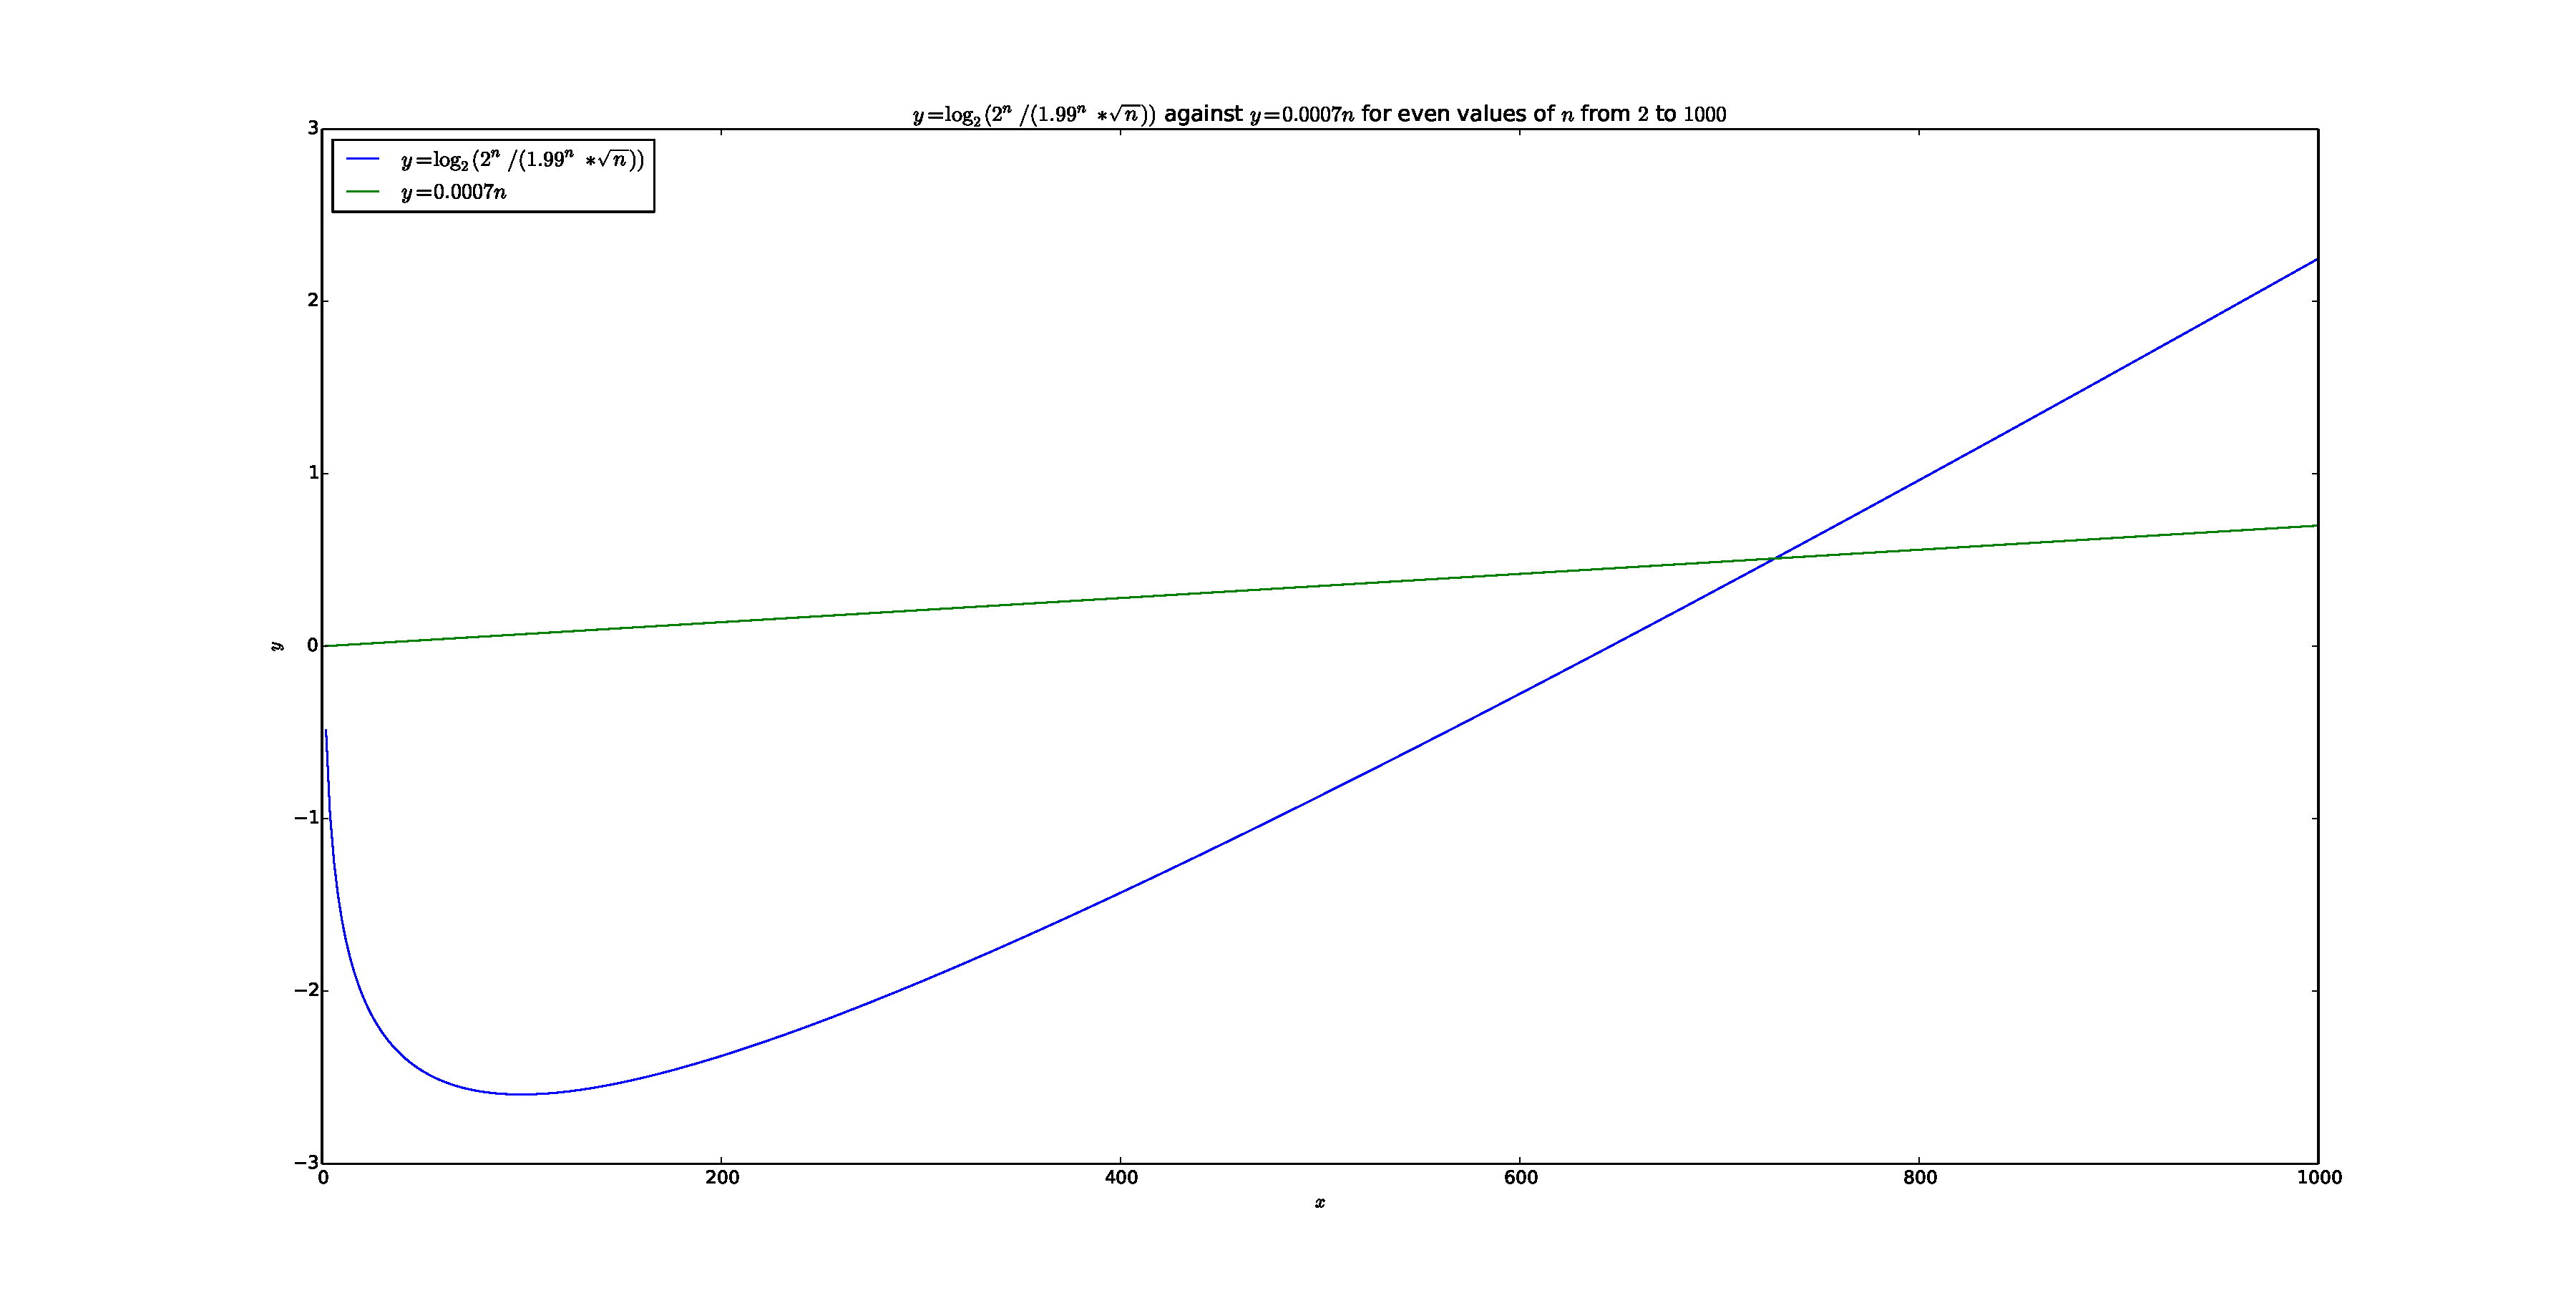
\includegraphics[width=\linewidth]{ddj_bound}
            \caption{Plot of lower bounds of Distributed Deutsch-Jozsa for $n \in \{2, 4,..., 998, 1000\}$}
            \label{fig:ddj-bound}
        \end{figure}

\end{document}
